\section{Постановка задачи}

Целью данной работы является построение алгоритма, который решает задачу сегментации снимков МРТ сердца. Задача сегментации заключается в том, чтобы определить, какие части изображения принадлежат целевому объекту, а какие нет. 

\subsection{Входные данные}

Каждый набор данных разделен на 3 части: 

\begin{itemize}
  \item данные для обучения
  \item данные для валидации
  \item данные для тестирования
\end{itemize}

Данные для обучения и валидации — это пары~$(\hat{X}_{train},\hat{Y}_{train})$ 
и~$(\hat{X}_{val},\hat{Y}_{val})$, 
где~$\hat{X}_{train} = \{\hat{x}_{train}^{i}\}, i\in{}\overline{1,n_{train}}$ 
и~$\hat{X}_{val} = \{\hat{x}_{val}^{i}\}, i\in{}\overline{1,n_{val}}$ соответственно 
— 2~упорядоченных набора матриц — снимков МРТ сердца, каждый элемент каждой из~которых 
представляет собой интенсивность соответствующего пикселя на снимке МРТ сердца, 
$\hat{Y}_{train}$ и~$\hat{Y}_{val}$ соответственно 
— 2 упорядоченных множества пар~$(x_{i},y_{i}), i = \overline{1,m}$, 
определяющие 2~соответствующих \mbox{$m$-угольника} 
— выделенные экспертом контуры сердца.

Данные для тестирования — упорядоченный набор 
матриц — снимков МРТ сердца~$\hat{X}_{test} = \{\hat{x}_{test}^{i}\}, i\in{}\overline{1,n_{test}}$, 
каждый элемент каждой из~которых представляет собой интенсивность соответствующего 
пикселя на~снимке МРТ сердца, для которого необходимо предсказать контур искомого объекта.

\subsection{Формальная постановка задачи}

Чтобы использовать нейронную сеть для решения задачи, преобразуем каждый 
набор~$\hat{X},\hat{X}\in{}\{\hat{X}_{train},\hat{X}_{val},\hat{X}_{test}\}$ 
в~соответствующий новый упорядоченный набор $X,X\in{}\{X_{train},X_{val},X_{test}\}$, 
каждый элемент которого — матрица~$R^{n\times{}n}$, каждый элемент которой, 
в~свою очередь, представляет собой нормализованную интенсивность соответствующего 
участка на~снимке МРТ сердца. Преобразование данных описано выражением~\eqref{eq:input_normalized},
где $X^{2}$ определяется~\eqref{eq:input_squared}, а~$E[X]$~—~\eqref{eq:input_expected_value}.

\begin{equation}
\label{eq:input_squared}
(X^{2})_{i,j}=((X)_{i,j})^{2}
\end{equation}

\begin{equation}
\label{eq:input_expected_value}
E[X]=\frac{
  \sum_{i,j}X
}{
  n^{2}
}
\end{equation} 

\begin{equation}
\label{eq:input_normalized}
X = \frac{
  \hat{X} - E[\hat{X}]
}{\sqrt{
  E[\hat{X}^{2}] - (E[\hat{X}])^2
}}
\end{equation}

Преобразуем каждый набор~$\hat{Y},\hat{Y}\in{}\{\hat{Y}_{train},\hat{Y}_{val}\}$ 
в~соответствующий упорядоченный набор~$Y,Y\in{}\{Y_{train},Y_{val}\}$, 
каждый элемент которого — матрица~$R^{n\times{}n}$. Каждый элемент последней, 
в~свою очередь, является числом~$1$~или~$0$, в зависимости от того, принадлежит~ли 
соответствующий пиксель заданному \mbox{$m$-угольнику} или~нет.

\begin{figure}[hb]
  \begin{center}
    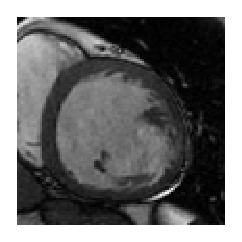
\includegraphics[width=0.3\textwidth,keepratio]{img/example-in}
    
\includegraphics[width=0.3\textwidth,keepratio]{img/example-out}
  \end{center}
  \caption{Пример данных для обучения}
\end{figure}

Таким образом, исходная задача сводится к задаче бинарной классификации каждого пикселя 
входного изображения — либо пиксель принадлежит объекту, либо~нет. На~вход алгоритму 
подаются нормализованные матрицы снимков МРТ, а~на~выходе алгоритма получается матрица, 
каждый элемент которой показывает вероятность принадлежности соответствующего пикселя объекту. 
Выход алгоритма затем сравнивается с~экспертной разметкой с~помощью различных метрик.

\subsection{Метрикa}

Чтобы оценить качество сегментации, введем метрику оценки качества сегментации. Результат сегментации 
можно представить либо~как~область пикселей, либо~как~контур вокруг этой~области. В~данной работе 
используется представление в~виде области пикселей и~индекс Дайса~\eqref{eq:dice_index} в~качестве метрики. 

\begin{equation}
\label{eq:dice_index}
  Dice(U,V) = \frac{2|U\cap{}V|}{|U| + |V|}
\end{equation}
